\documentclass{article}
\usepackage[utf8]{inputenc}
\usepackage{graphicx}
\usepackage{enumitem}

%Sets the languages
\usepackage[norwegian, english]{babel}

%Configuration of numbered list
\newlist{legal}{enumerate}{10}
\setlist[legal]{label*=\arabic*.}


\title{Kravspesifikasjon}
\author{}
\date{Oktober 2019}

\begin{document}

\maketitle

\section{Introduksjon}
\begin{figure}[h]
\centering 
    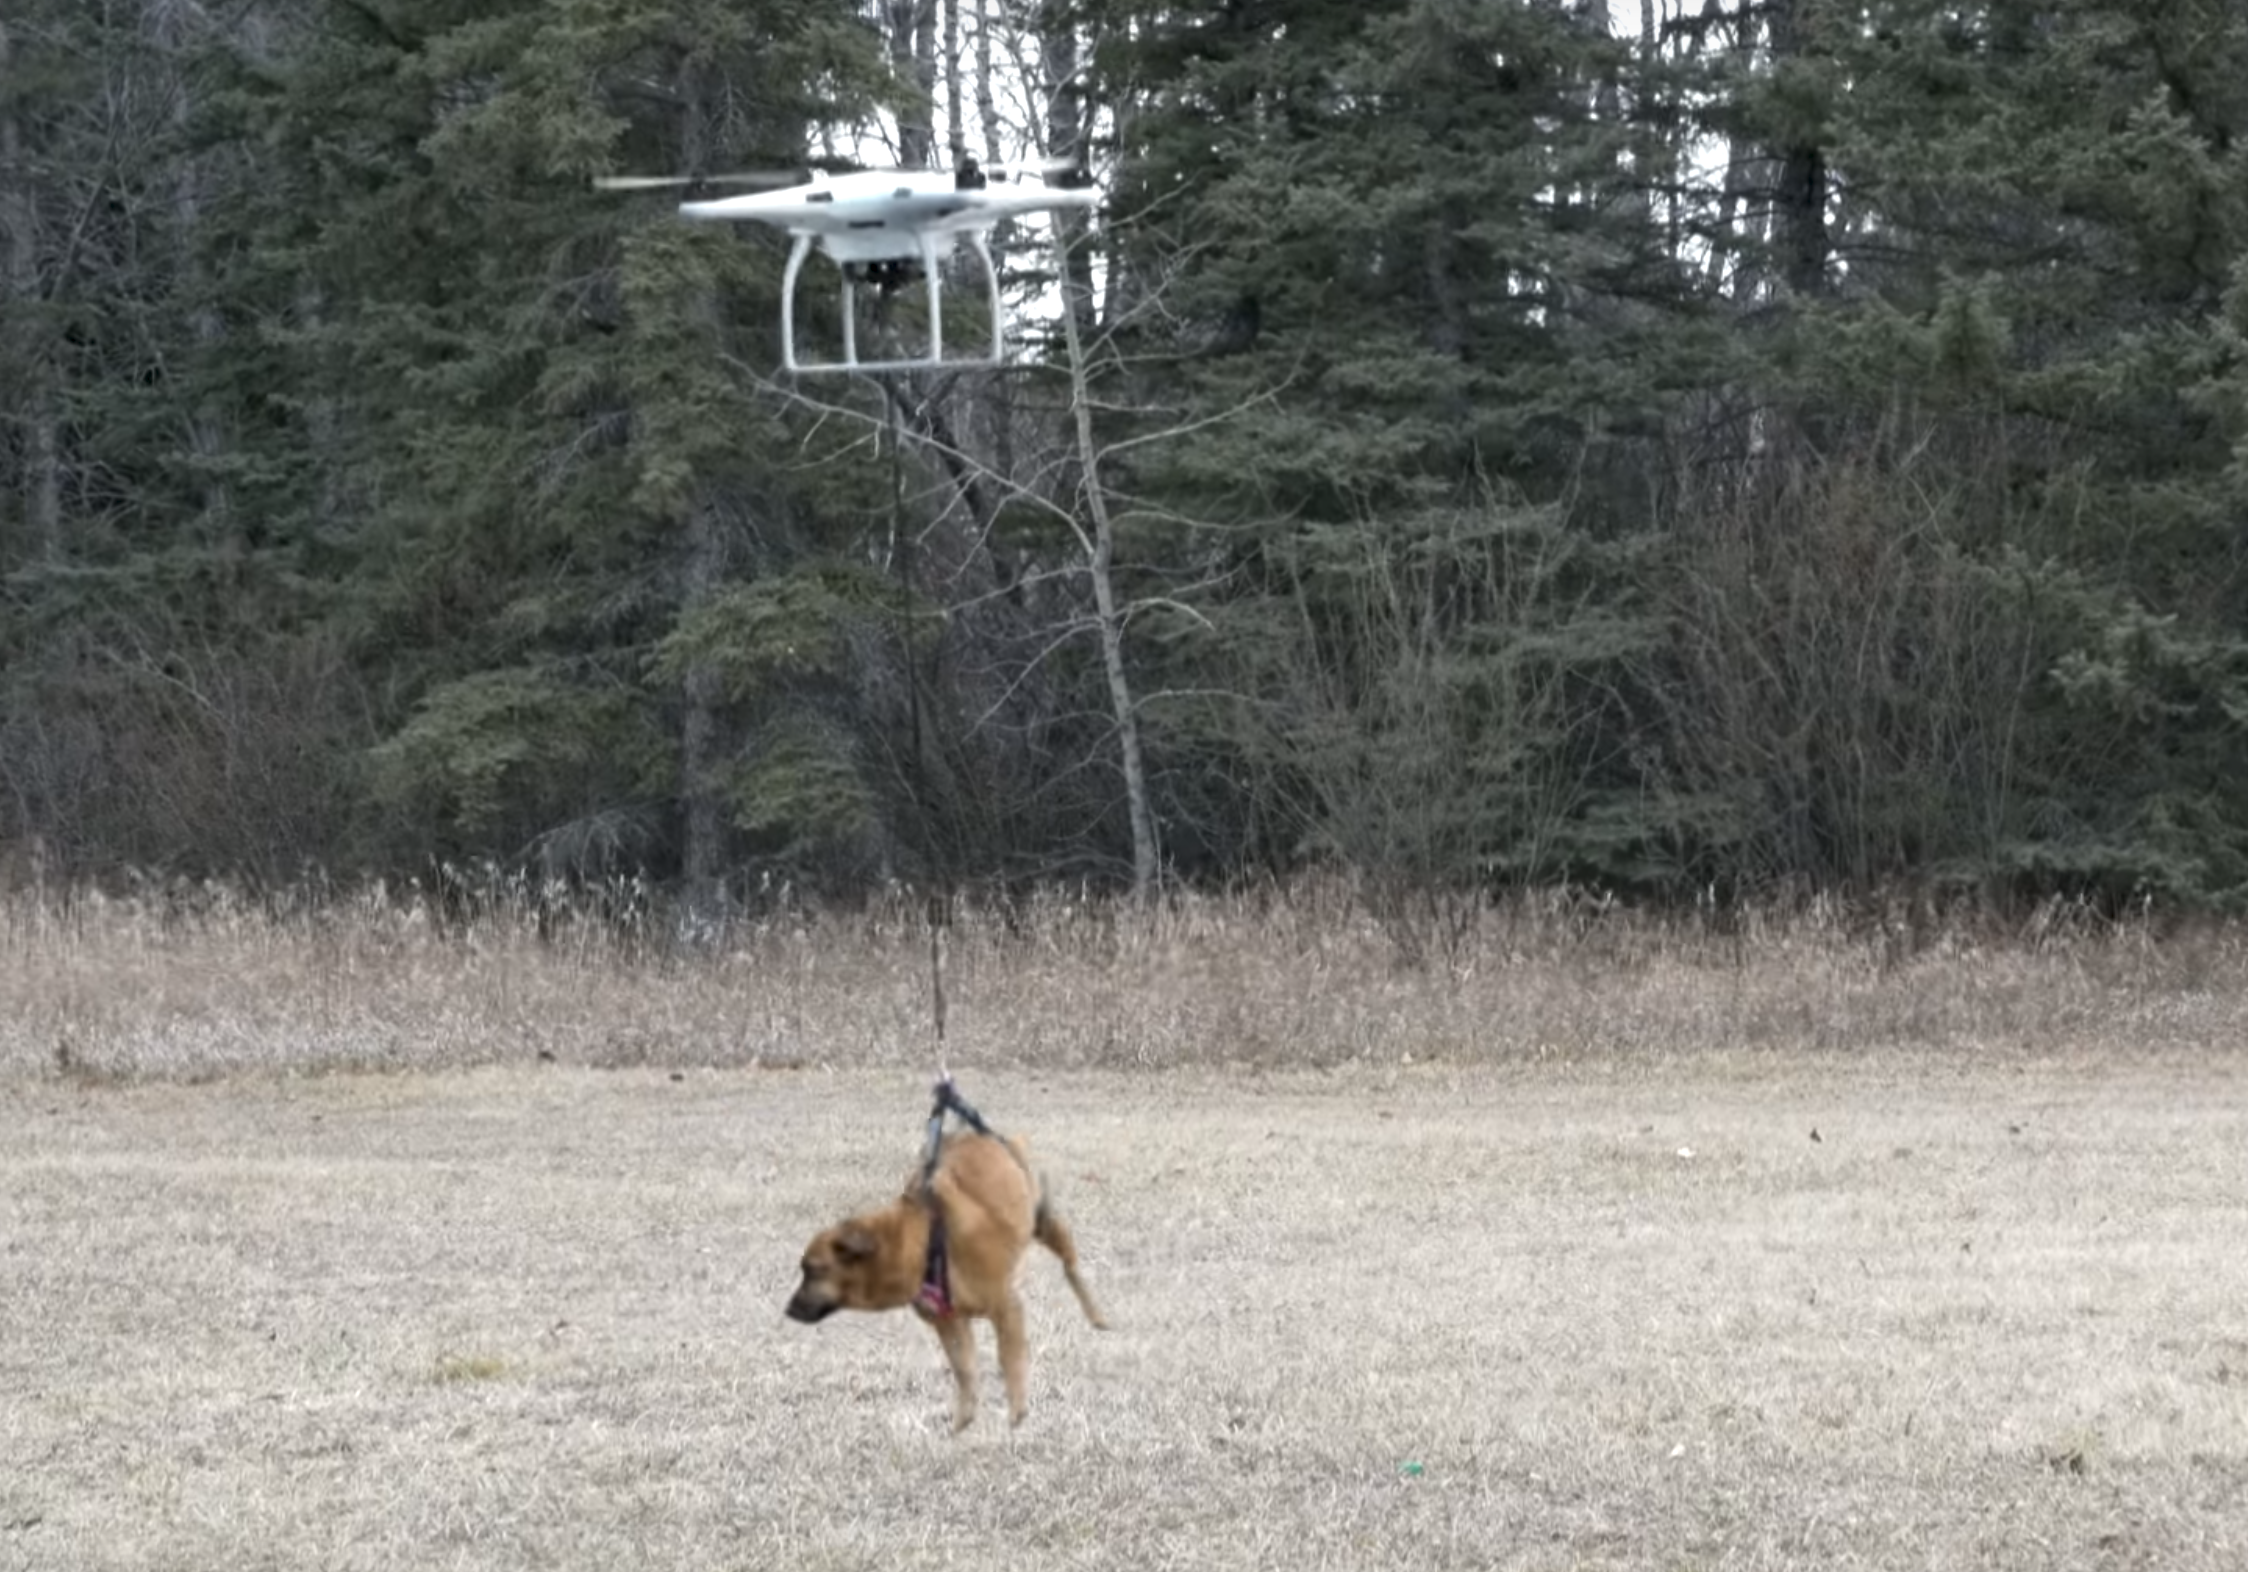
\includegraphics[scale=0.1]{images/dog}
    \caption{Front view of Sea King helicopter at Rygge Airbase. Photo taken by Gjermund Østensvig.}\label{fig:Seaking1}
\end{figure}

Bilde test \ref{fig:Seaking1}

\section{Funksjonelle Krav}

\begin{legal}
    \item Webside
    \begin{legal}
        \item Bruker, klubb og admin skal kunne se kalender for inneværende måned med arrangementer og trykke seg tilbake til forrige måned eller frem til neste måned
    \end{legal}
    \item Applikasjon
    \begin{legal}
        \item Klubb og administrator skal kunne logge inn på applikasjonen ved hjelp av å trykke en knapp (skal ikke kunne logge inn i webgrensesnittet)
        \item Klubb skal kunne legge til kommende arrangementer
        \end{legal}
        \item 
    \end{legal}
    \item API
    \begin{legal}
        \item Systemet skal autogenerere utøverprofiler basert på resultater fra arrangement
        \item API-et skal kunne ta i mot tabeller med data og importere det til database
    \end{legal}
    \item Database
    \begin{legal}
        \item 
    \end{legal}
    \item
\end{legal}
\end{document}
